\chapter{Results}\label{chap:fourth chapter}

The results of this experiment can be broadly classified into 2 categories, namely simulation results and those of the real system. The following chapter looks into these results in detail.


\section{Simulation Results}

To test the accuracy of the model and the speed of the optimization algorithm, simulations were performed and studied.

For the implementation of the MPC algorithm, the simulation was conducted on the PC, with a simulated pendulum class with internal functions that simulate the behavior of a real pendulum. 

\begin{figure}[H]
	\centering
	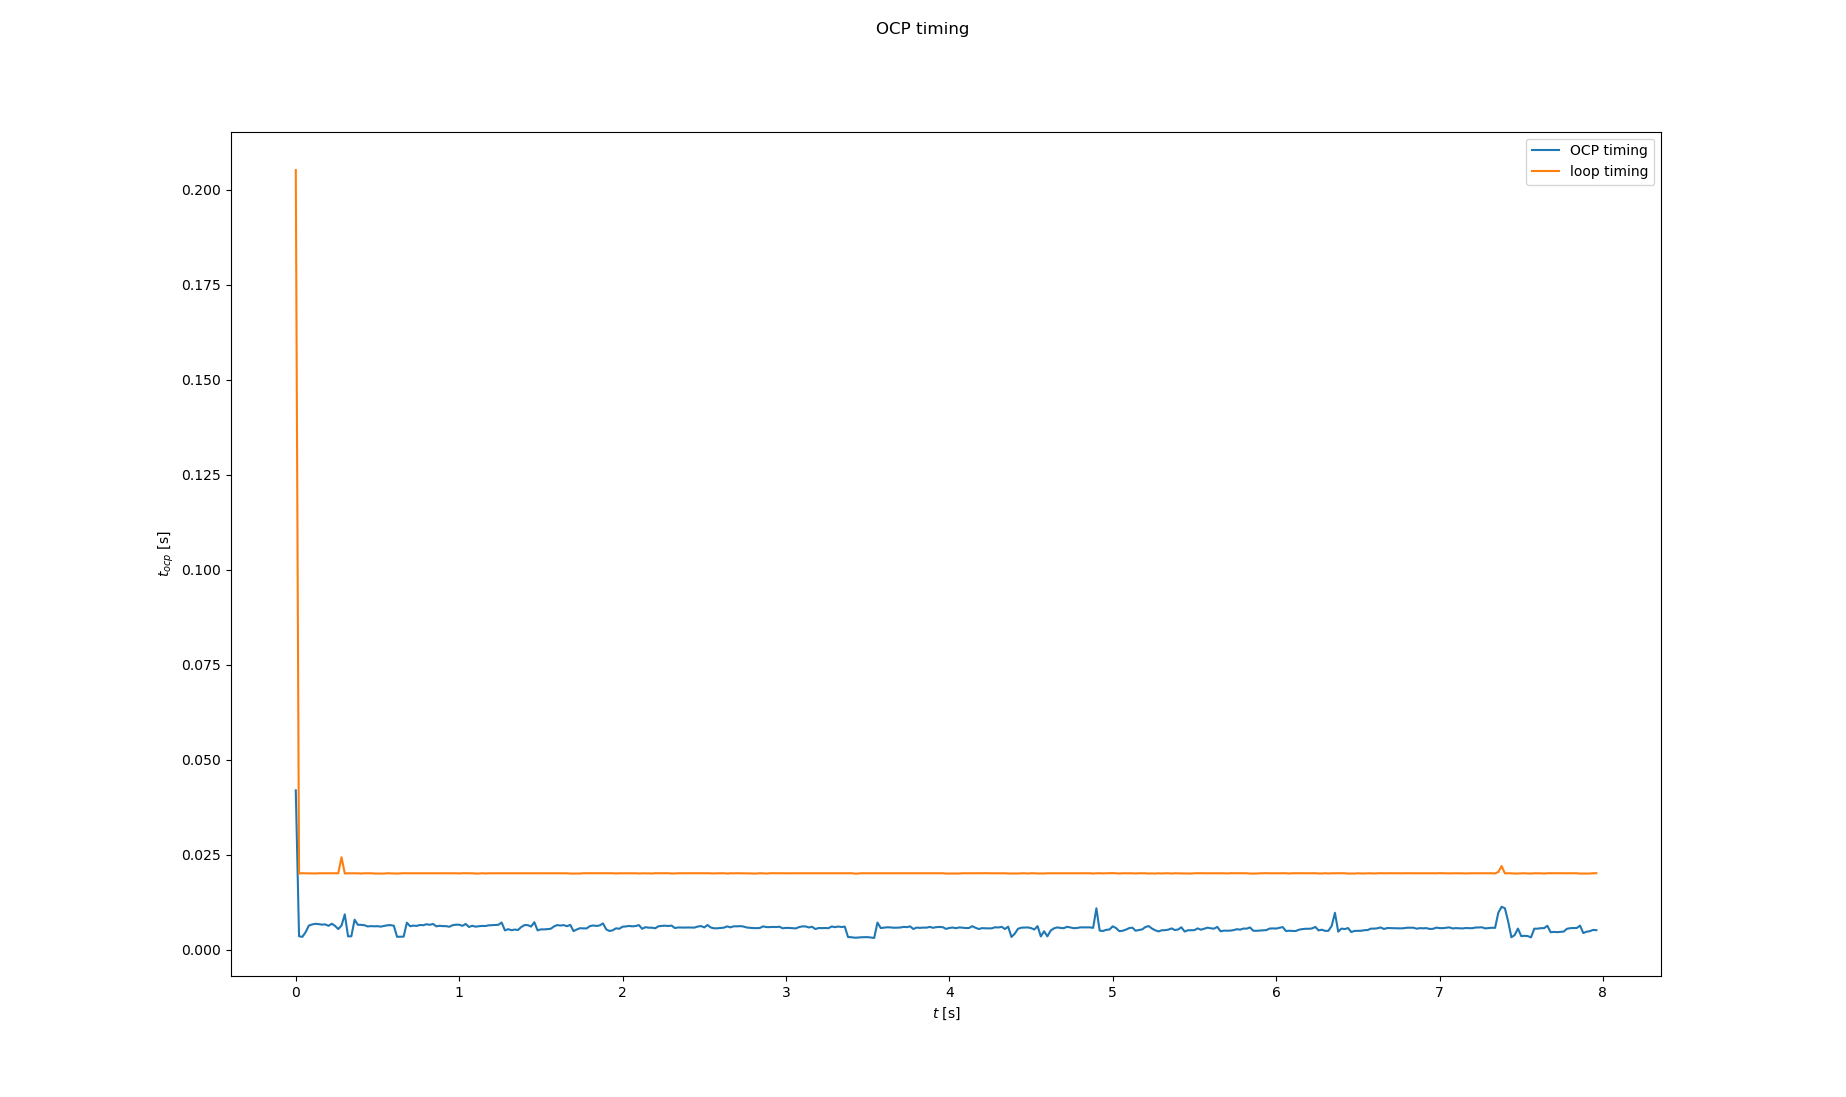
\includegraphics[width=0.96\textwidth]{"src/Images/OCP_Timing_Graph_Pendulum_Simulation.png"}
	\caption{Timing graph: Simulation}
	\label{fig:Timing: Pendulum simulation}
\end{figure}

A necessary condition for proper functioning of the real system is that the measurement of states and the calculation, application of the input must happen within the sampling time of the controller, which is \textbf{20} ms in our case. 

Figure \ref{fig:Timing: Pendulum simulation} depicts the time taken to solve the OCP at every iteration of the main loop and it is solved in less than 10 milliseconds at almost every iteration, which leaves enough time to communicate with the pendulum.


\begin{figure}[H]
	\centering
	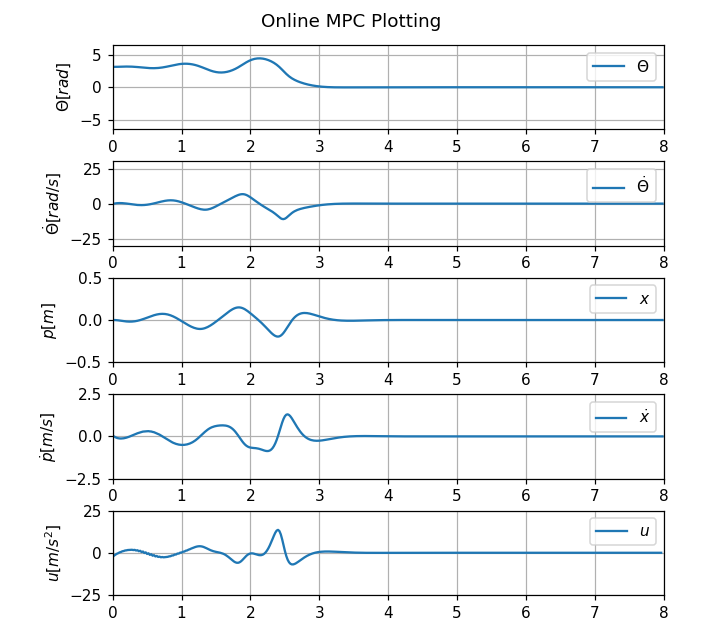
\includegraphics[width=\textwidth]{"src/Images/PC_Simulation_OnlinePlot.png"}
	\caption{Simulation}
	\label{fig:Simulation}
\end{figure}

Figure \ref{fig:Simulation} depicts the states during the MPC algorithm which converges to the origin as is expected.  
 
 \clearpage
 
\section{Real system results}

Upon running the algorithm on the real system, the following results were obtained:

\begin{figure}[H]
	\centering
	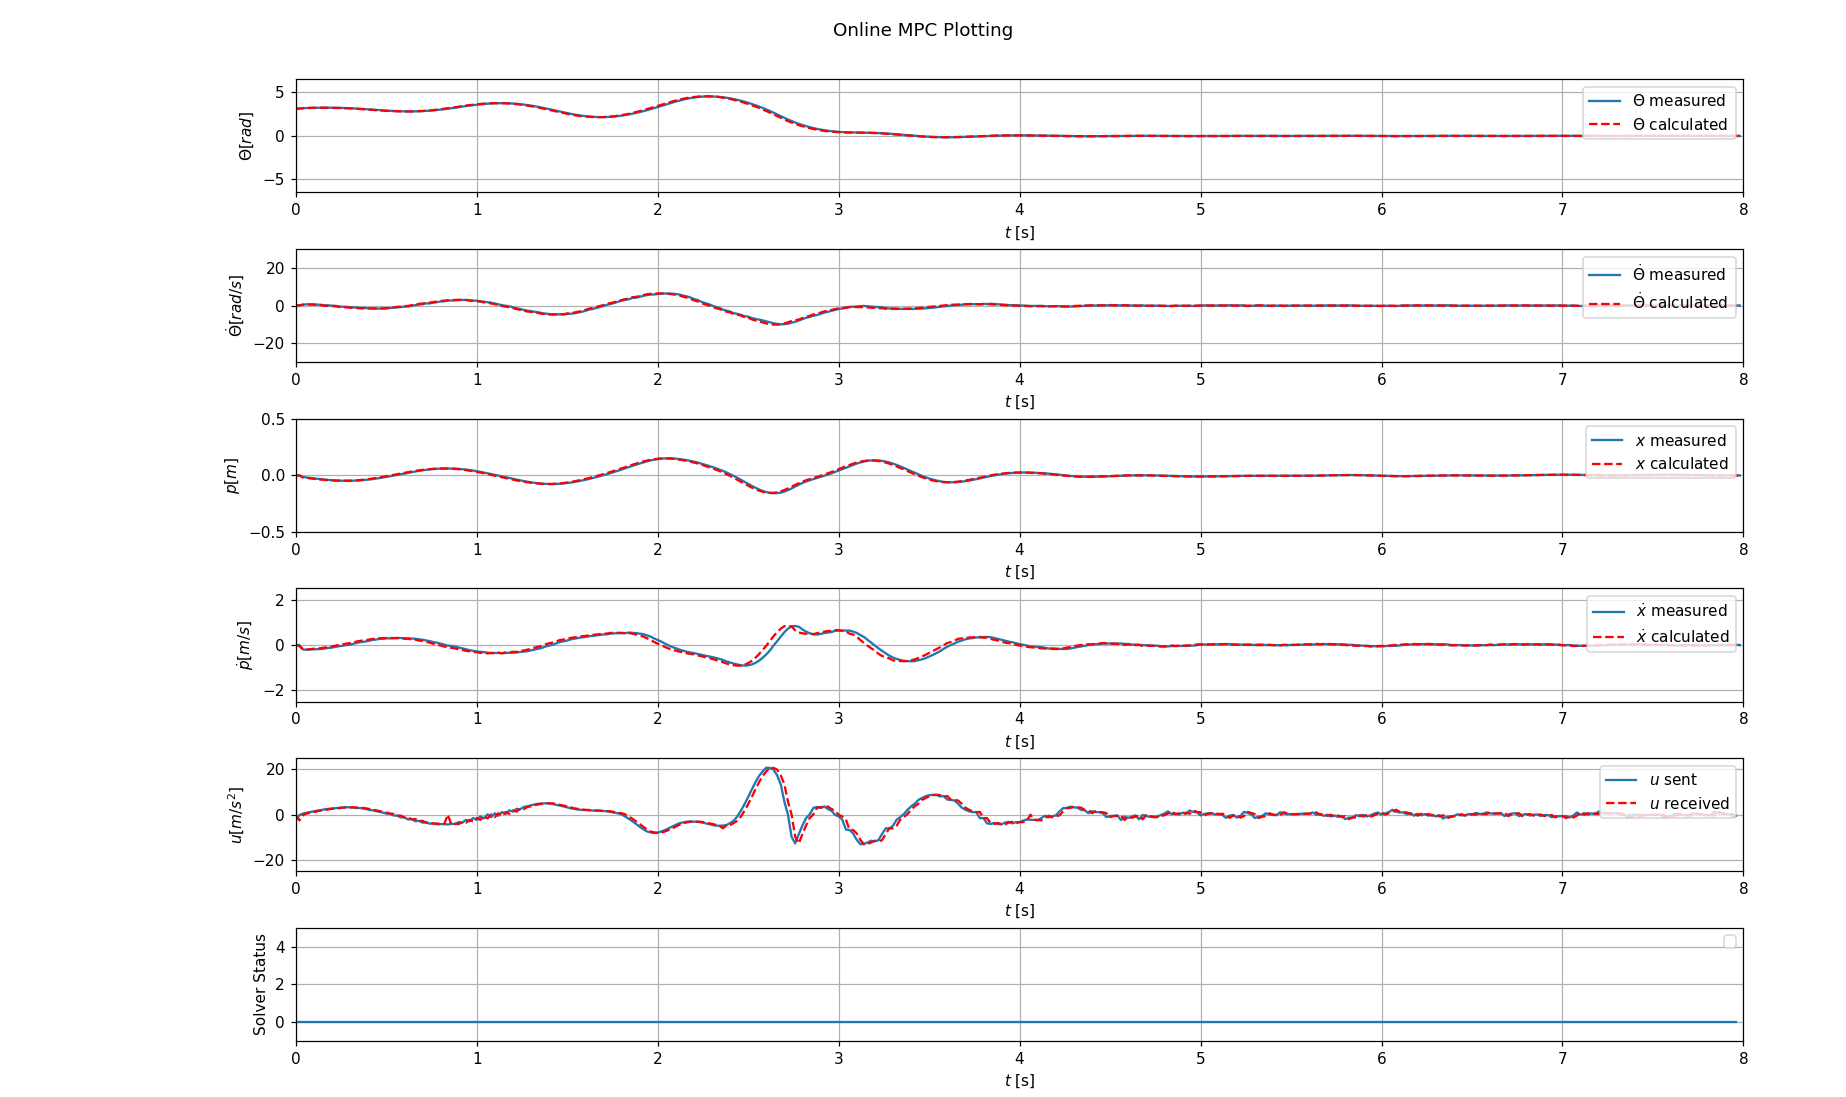
\includegraphics[width=\textwidth]{"src/Images/Real_Pendulum_OnlinePlot.png"}
	\caption{Real Pendulum}
	\label{fig:Real Pendulum Plot}
\end{figure}

As seen here, the states closely converge to the origin and therefore the pendulum stabilizes in an upright position within 3.5-4 seconds. There are also slight disturbances on the input which is expected due to real world factors such as different friction coefficients and drag. 


